% This material is copyright Simon Dobnik and made available under the
% Creative Commons Attribution 4.0 International License (CC-BY-SA)
% license http://creativecommons.org/licenses/by-sa/4.0/
% 
% Email: simon.dobnik@gu.se
% Web: http://dobnik.net/simon/teaching/shared/LT2112-formling/


\documentclass{beamer}


\usepackage{graphicx,hyperref,lingmacros,qtree,stmaryrd,fullname}
\usepackage[utf8]{inputenc}





\logo{
\includegraphics[height=0.5cm]{pics/GU-logo.pdf}} 

\newcommand{\bblue}[1]{{\usebeamercolor[fg]{frametitle}{#1}}}



\definecolor{links}{HTML}{2A1B81}
\hypersetup{colorlinks,linkcolor=,urlcolor=links}


\setbeamertemplate{footline}[frame number]


\resetcounteronoverlays{enums}


\AtBeginSection[]
{
\begin{frame}[plain]

{\huge\bblue{\insertsectionhead}}

\end{frame}
}



\setlength\fboxrule{1pt}
\setlength\fboxsep{0mm} 



\newcommand{\evaluation}[2][]{\ensuremath{\llbracket #2\rrbracket^{#1}}}
\newcommand{\semval}[1]{\evaluation[v]{\text{#1}}} 

\newcommand{\lb}[1]{[$_{\textsf{#1}}$} 


\newcommand{\mng}[1]{\mbox {$[ \! [$ #1 $] \! ]$}}





\title[Semantics]{L7: Semantics I - Meaning}

\author[Dobnik]{Simon Dobnik \\ 
Department of Philosophy, Linguistics and Theory of Science
} 

\date{October 1, 2015}





\begin{document}





\frame{\titlepage}





\section{Introduction to semantics}

\frame{

\frametitle{What is semantics?}

The study of \bblue{linguistic meaning} and \bblue{interpretation of linguistic expressions}.

\bigskip

\pause








But what is meaning?

\enumsentence{He is the Prime Minister. \\
In 2013 true with he = Fredrik Reinfeldt \\
In 2015 true with he = Stefan Löfven
}

\begin{itemize}

\item \bblue{Utterances:} unrepeatable speech or writing events at a particular point in space and time

\item \bblue{Sentences:} linguist's abstractions from utterances: \\
``a contextually identified male is the PM''

\end{itemize}


}





\frame{


\frametitle{Semantics and Pragmatics}

\bblue{Speaker's meaning:} the speaker intends to convey something extra with the utterance

\enumsentence{I'd like a glass of water.}

\bigskip

Contextual and inferential

\begin{itemize}

\item In a restaurant: a request or command.

\item Hiking in the mountains on a very hot day: an expression of desire.

\end{itemize}

Language is always produced in context


}





\frame{

\frametitle{Semantics or pragmatics}

\bblue{Semantics:} study of meaning of linguistic expressions

\bigskip

\bblue{Pragmatics:} the study of meaning related to the situated use of linguistic expressions: the status of utterances (rather than sentences) and their effects.




}





\begin{frame}

\frametitle{Literal and non-literal meaning}

\bblue{Metaphors:}

\eenumsentence{

\item letting the cat out of the bag

\item put the foot down

\item chicken or the egg

}

\end{frame}






\frame{

\frametitle{The significance of language}

What does language (i.e. sentences) mean? What is the meaning about?

\bigskip

\bblue{Informational significance:} meaning is a link between linguistic expressions and things in the world.

\bigskip

\bblue{Cognitive significance:} meaning is a link between linguistic expressions and human mental constructs.

}





\frame{

\frametitle{Informational significance}


\bblue{Referential theories:} regular correspondences between linguistic expressions and the world, e.g. \bblue{Truth-conditional semantics}.

\bigskip

\enumsentence{The door is closed.}

\bigskip

Corresponds to an infinity of somehow related situations.

\bigskip

The nature of correspondences:

\begin{itemize}
  \item not predetermined by the structure of the environment;   \item perception and reasoning is involved.
\end{itemize}


}





\frame{

\frametitle{Cognitive significance: reference to private internal worlds}

\begin{itemize}

\item The hearer can judge what mental state this refers to: \enumsentence{Joan wants a tomato sandwich.}

\item Can communicate about our internal experience.

\end{itemize}

\bigskip

Regular correspondences between linguistic expressions and cognitive processes and states in the brain (without considering relations to situations), e.g. \bblue{representationalists}.


}


















\frame{

\frametitle{The productivity of linguistic meaning}

\begin{itemize}

\item NL syntax produces infinite number of sentences.

\item Each sentence has a meaning: infinite number of meanings.

\item We know the meaning of words.

\item How to combine meanings of words to more complex meanings?
\eenumsentence{\item 1437.952 + 21.84
\item I saw a pink whale in the parking lot.}


\end{itemize}

}





\begin{frame}

\frametitle{Compositionality}

The principle of compositionality: the meaning of a complex expression is determined by the meanings of its constituent expressions and the rules used to combine them

\begin{center}

\fbox{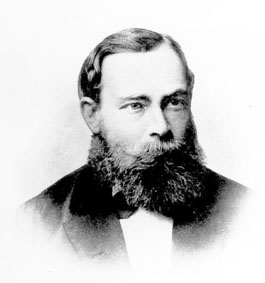
\includegraphics[width=.375\textwidth]{./pics/frege.jpg}}

\end{center}

(\href{http://en.wikipedia.org/wiki/Gottlob_Frege}{Gottlob Frege}, a logician (2nd half on C19 and early C20).


\end{frame}





\frame{

\frametitle{A brief history of formal semantics}

End of 1960s: \href{http://en.wikipedia.org/wiki/Richard_Montague}{Richard Montague}, philosopher at University of California Los Angeles (UCLA): introduced logic for the study of linguistic meaning


\begin{center}

\fbox{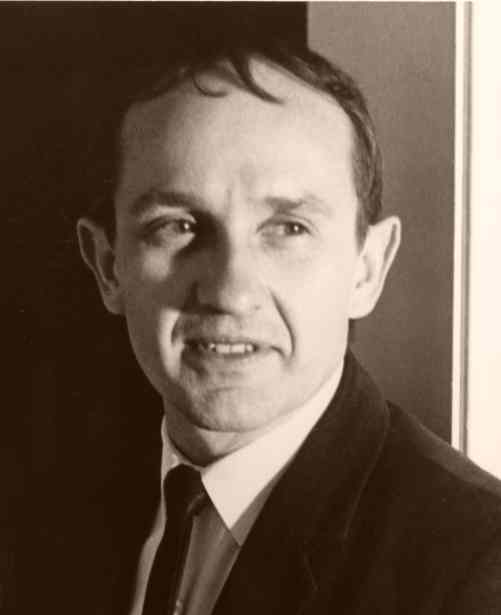
\includegraphics[width=.375\textwidth]{./pics/montague.jpg}}

\end{center}

}





\frame{

\frametitle{A brief history of semantics}

\href{http://en.wikipedia.org/wiki/Barbara_Partee}{Barbara Partee}, linguist and philosopher at UCLA introduced this approach to linguistics: \bblue{Montague grammar} or \bblue{Montague semantics}

\begin{center}

\fbox{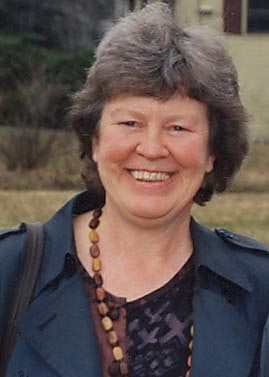
\includegraphics[width=.33\textwidth]{./pics/partee.jpg}}

\end{center}





}





\frame{

\frametitle{A brief history of semantics}

Developed in 1970s and 1980s as a research area.

\bigskip

Many computational approaches appeared in the 1990s and beyond: Patrick Blackburn and Johan Bos

\begin{center}

\fbox{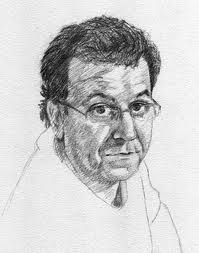
\includegraphics[width=.33\textwidth]{./pics/blackburn.jpg} 
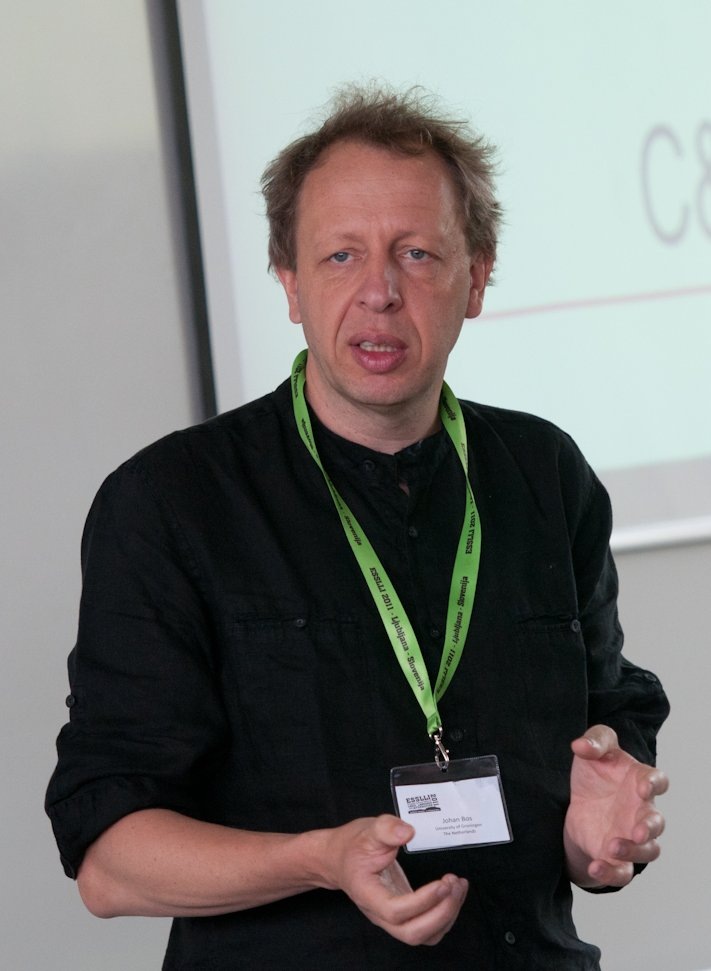
\includegraphics[width=.305\textwidth]{./pics/bos.jpg}}

\end{center}

}
























\section{Meaning}

\frame{

\frametitle{Denotation}

The name \bblue{denotes} denotation, denotatum, reference, or semantic value.

\bigskip

\bblue{Pavarotti:} a certain person with this name

\bigskip

Other NPs have similar denotations:

\eenumsentence{\item It is a pencil.
\item This is yellow.
\item The tallest man in the world lives in Los Angeles.
\item ?The present queen of France is smart. \item ?The book that Agatha Christie wrote is about Hercule Poirot.} 

}





\frame{

\frametitle{NPs are more complicated in terms of denotation}

\begin{itemize}

\item Distributive and collective reading of sets of individuals

\eenumsentence{\item The students in my class are Swedish.
\item The students in my class outnumber those in yours.}

\item \pause Substances

\enumsentence{Gold is expensive}

\item \pause Actions

\enumsentence{Running is healthy.}

\item \pause Abstract entities

\enumsentence{Justice should be prised.}

\item \pause Fictional characters

\enumsentence{Bond is my hero.}
\end{itemize}


}





\frame{

\frametitle{A theory of individuals}

\enumsentence{The table cannot be identified as the sum of partitions of matter that make it up at a given time: all parts may be replaced through repairs and we would still identify it as a table.}


\begin{itemize}

\item A theory of individuation is required.

\item We can work with the notion of individuals here.

\end{itemize}

}





\frame{

\frametitle{The denotation of quantified NPs}



\enumsentence{A/some student in my class is blond. \\ An individual from the class or a set of students is blond. }

\enumsentence{Every student is blond. \\ Every individual from the class or a set of students (the entire class of students) is blond.}

\enumsentence{No student in my class is blond. \\ No individual from the class or a set of students is blond.}

\enumsentence{//Every student outnumbers the professors. \\ //The class of students outnumbers the professors.} 
}





\frame{

\frametitle{The denotation of quantified NPs}

Interaction with negation:

\eenumsentence{\item Every Italian doesn't like Pavarotti.
\item //The class of Italians doesn't like Pavarotti.
\item Not every Italian likes Pavarotti.
\item Every Italian dislikes Pavarotti.} 

\bigskip \pause

The choice of individuals - random?

\eenumsentence{\item In my class, a woman is blond and a woman is red-haired and \ldots \item Every man loves a woman. }

}

























\frame{

\frametitle{Productivity of meaning}

\begin{itemize}

\item What do other linguistic categories denote?

\item How does the reference of complex expressions depends on the reference of their components?

\end{itemize}

\pause

\bigskip

\enumsentence{Pavarotti is an Italian singer.}

\begin{itemize}

\item \semval{Pavarotti}: an individual

\item \semval{is an Italian singer}: a property denoting a state of affairs or a situation

\item \semval{Pavarotti is an Italian singer}: a situation where a certain individual has a property of being an Italian singer

\end{itemize}

}





\frame{

\frametitle{Productivity of meaning}

\enumsentence{No woman smokes.}

\begin{itemize}

\item \semval{no woman}: no denotation

\item \semval{smokes}: property 

\item \semval{no woman smokes}: situation where no individual from the class of women has the property of smoking

\end{itemize}

}





\begin{frame}

\frametitle{Non-existing, hypothetical situations}


\eenumsentence{\item Pavarotti is French. \item If Pavarotti sings ``O che gelide manine,'' I want to be there.}

\end{frame}

















\frame{

\frametitle{The meaning of sentences}

\begin{itemize}

\item We never deal with labels and objects in isolation.

\item Even\ldots
\eenumsentence{\item Pavarotti! (pointing at a person)
\item This person is Pavarotti.} 
\item Frege: Nur im Zusammenhange eines Satzes bedeuten die Wörter etwas - Only in the context of a sentence do words have meaning.



\item Well-formed structures expressing thoughts/propositions referring to/denoting whole situations.


\item True or false 
\end{itemize}

}























\frame{

\frametitle{Tarski (1935, 1944)}

S is true if conditions that S claims to obtain do obtain. 
\bigskip

\enumsentence{S is true in v iff (if and only if) p. (T-sentence)}\label{t-sentence}

\begin{itemize}

\item S: a structural description of a language L

\item v: a situation, a specification of facts

\item p: the conditions for S to be true in v \\ the truth conditions for S. 
\end{itemize}







}





\frame{

\frametitle{Inference}

We must be able to model \bblue{entailment}:

\eenumsentence{\item\label{entail1} Pavarotti is an Italian singer.
\item\label{entail2} Someone is an Italian singer.}

\begin{itemize}

\item Situation denoted by (\ref{entail2}) is contained in the situation denoted by (\ref{entail1}).

\item Whenever situation denoted by (\ref{entail1}) occurs, the situation denoted by (\ref{entail1}) also occurs.

\item Whenever (\ref{entail1}) is true, (\ref{entail1}) is true.

\end{itemize}



}





\frame{

\frametitle{Sense and reference}

\begin{itemize}

\item Two expressions that entail each other have the same reference.

\eenumsentence{\item the sister of John
\item the daughter of John's parents}


\item If we have an expression A containing an expression B and we replace B in A with an expression C that has the same reference as B, the reference of A does not change.

\eenumsentence{\item the sister of John
\item the sister of Mary's husband}

\end{itemize}


}





\frame{

\frametitle{Reference and entailment of sentences}

If a sentence is true, it's truth value is true (T) or false (F).

\eenumsentence{\item\label{tval1} Pavarotti is cute. \item\label{tval2} The truth value of ``Pavarotti is cute'' = T. \item\label{tval3} The truth value of ``It snows'' = T
\item\label{tval4} It snows.}

\begin{itemize}

\item (\ref{tval1}) and (\ref{tval2}) have the same reference and hence entail each other 
\item (\ref{tval2}) and (\ref{tval3}) entail each other due to replacement with a co-referential expression 
\item (\ref{tval3}) and (\ref{tval4}) entail each other

\end{itemize}

Two arbitrary sentences with the same truth value have the same reference! 

}





\frame{

\frametitle{Meaning = sense + reference}

\begin{itemize}

\item Sentences are \bblue{describing situations} not only \bblue{referring
  to them}. 
\item Gottlob Frege: \bblue{reference} or \bblue{Bedeutung} and \bblue{sense} or \bblue{Sinn}

\item Carnap (1947): \bblue{intension} and \bblue{extension}

\end{itemize}


\bigskip 

NPs: ``the morning star'':

\begin{itemize}

\item \bblue{sense:} the concept of a star that disappears last in the morning

\item \bblue{reference:} Venus

\end{itemize}

}





\frame{

\frametitle{Sense and reference}

NPs: ``the evening star'':

\begin{itemize}

\item \bblue{sense:} the concept of a star that appears first in the evening

\item \bblue{reference:} Venus

\end{itemize}


\bigskip \pause

VPs: ``is Italian'':

\begin{itemize}

\item \bblue{sense:} the concept of being Italian

\item \bblue{reference:} a set of all individuals who are Italian

\end{itemize}


\bigskip \pause

S: ``Pavarotti is Italian'':

\begin{itemize}

\item \bblue{sense:} the thought/proposition that Pavarotti is Italian

\item \bblue{reference:} True

\end{itemize}

}





\begin{frame}

\frametitle{Further reading}

\cite{Chierchia:2000uq}, Chapter 2, Denotation, Truth, and Meaning.

\end{frame}





\begin{frame}[allowframebreaks]{References}

\small


\bibliographystyle{fullname}
\bibliography{bibliography}

\end{frame}





\end{document}


